\documentclass[paper=a4, fontsize=12pt]{scrartcl}

\usepackage{graphicx}
\usepackage{siunitx}
\usepackage{amsmath}
\usepackage{mathrsfs}
\usepackage{float}
\usepackage{subfig}
\usepackage{verbatim}
\graphicspath{{./img/}}

\title{
	\normalfont \normalsize
	\textsc{University of Ottawa} \\ [5pt]
	\huge Discrete-Velocity Scheme Project
}
\author{Mathieu Marchildon} % Your name
\date{\normalsize \today} % Today's date or a custom date


\begin{document}
\maketitle


\section{Shock-Tube Problem}
For the initial conditions of the shock-tube we must select an appropriate velocity space.
This velocity space can be determined by observing the distribution function on each side of
the shock tube for both initial conditions.
The distribution function in velocity space can be determined by applying Maxwell-Boltzmann distribution
for various ranges in velocity space.
\[
        f = \frac{\rho}{m} \Big( \frac{\rho}{2 \pi p}\Big)^{\frac{1}{2}}e^{\frac{\rho}{2 p}(u-v)^2}
\]
\begin{figure}[H]%
    \centering
    \subfloat[Left initial conditions]{{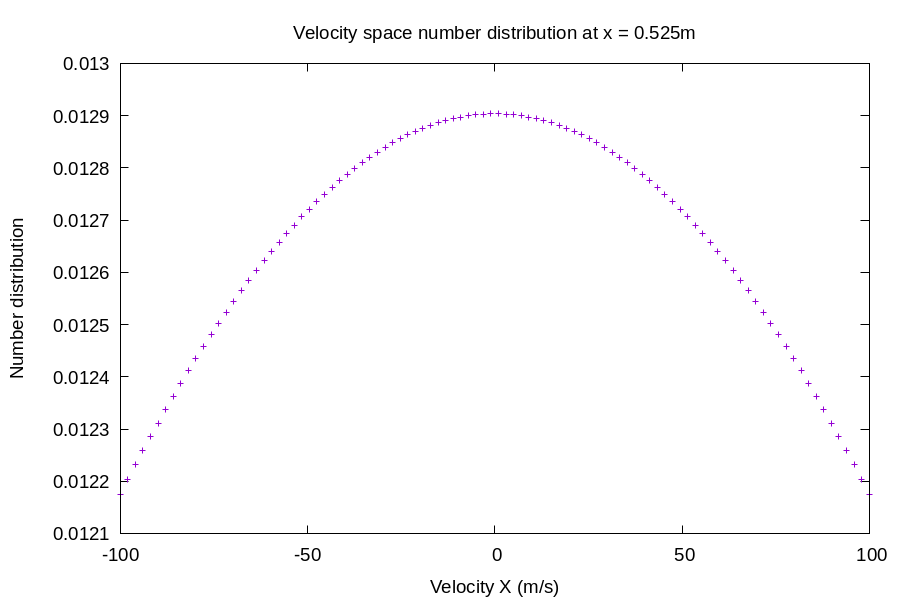
\includegraphics[width=7cm]{left_init_100} }}%
    \qquad
    \subfloat[Right initial conditions]{{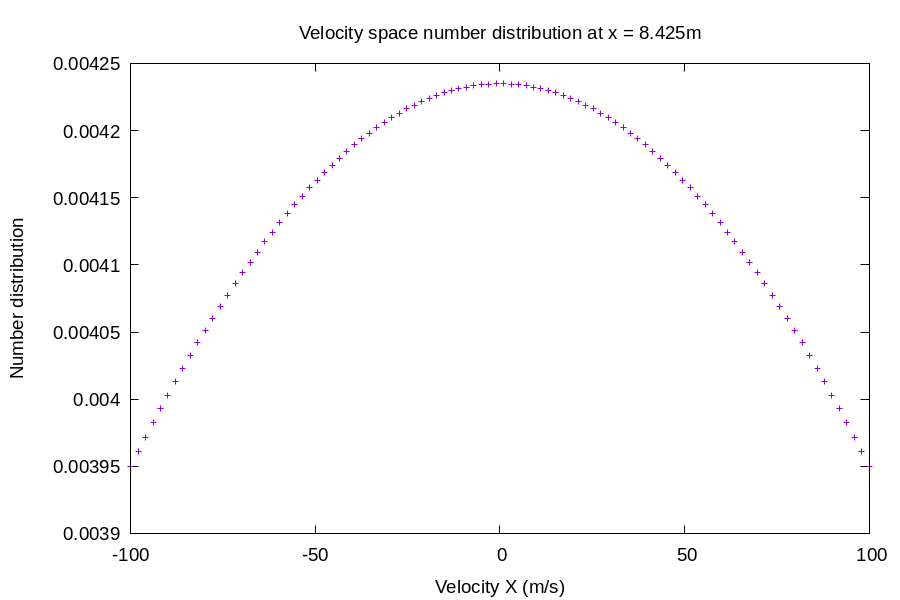
\includegraphics[width=7cm]{right_init_100} }}%
    \caption{Distribution function at initial conditions \newline velocity range of $\pm \SI{100}{\meter \per \second}$
 }
    \label{fig:init_100}%
\end{figure}

\noindent
Figure \ref{fig:init_100} shows the distribution function for the left and right initial conditions.
The velocity space selected was ranging from $\pm \SI{100}{\meter \per \second}$.
This range of velocity as shown in Figure \ref{fig:init_100} is insufficient as the tail
end of the distribution is cut off for both the left and right ends of the shock tubes.
\begin{figure}[H]
    \centering
    \subfloat[Left initial conditions]{{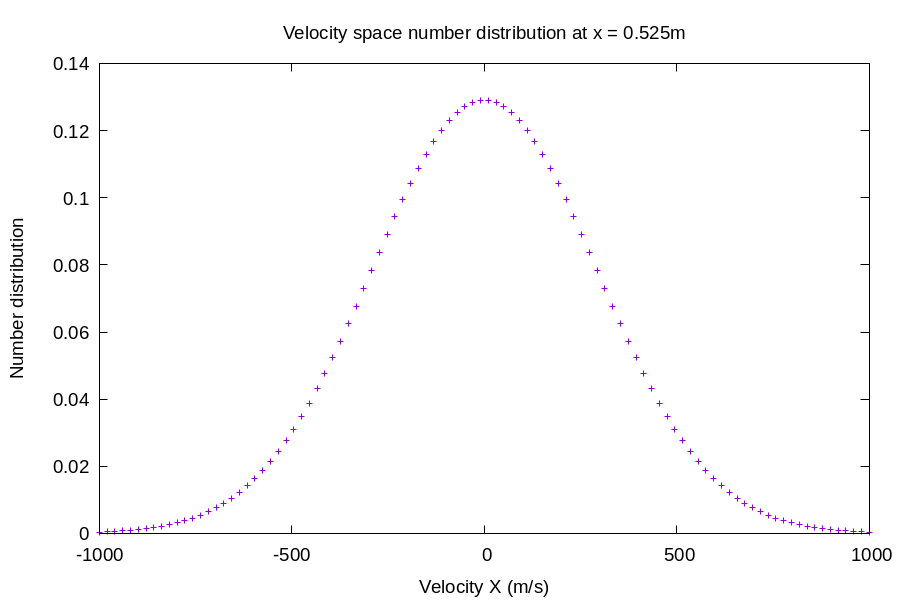
\includegraphics[width=7cm]{left_init_1000} }}%
    \qquad
    \subfloat[Right initial conditions]{{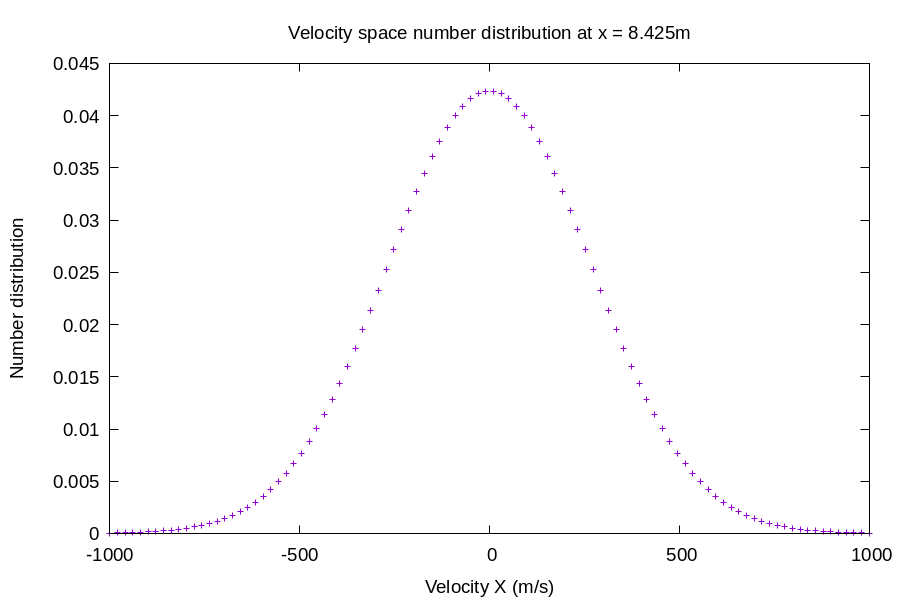
\includegraphics[width=7cm]{right_init_1000} }}%
    \caption{Distribution function at initial conditions \newline velocity range of $\pm \SI{1000}{\meter \per \second}$
 }
    \label{fig:init_1000}
\end{figure}

\noindent
Selecting a velocity range of $\pm \SI{1000}{\meter \per \second}$, as shown in \ref{fig:init_1000} we obtain
a velocity space that covers the full distribution of the particle space.


In addition to verifying the velocity space distribution we can also evaluate the properties of the gas
at those initial conditions.
The properties of the gas can be computed at each point in the $x$ direction by the following equations.

\begin{align*}
        \rho &= \langle m F \rangle  &  c = v-u\\
        \rho u &= \langle m v F \rangle \\
        p &= \langle m c^2 F \rangle \\
        q &= \frac{1}{2}\langle m c^3 F \rangle \\
\end{align*}

\begin{figure}[H]
    \centering
    \subfloat[Left initial conditions]{{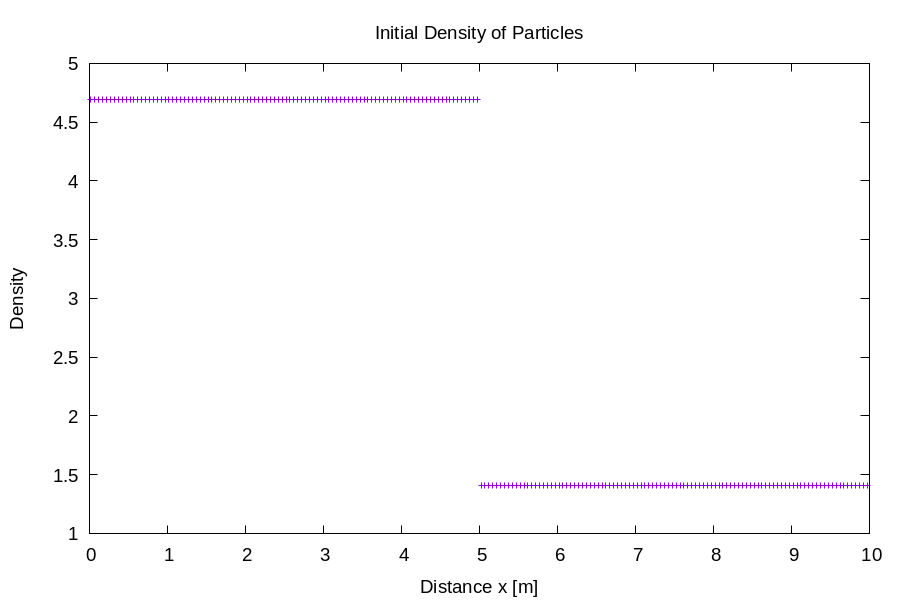
\includegraphics[width=7cm]{init-rho} }}%
    \qquad
    \subfloat[Right initial conditions]{{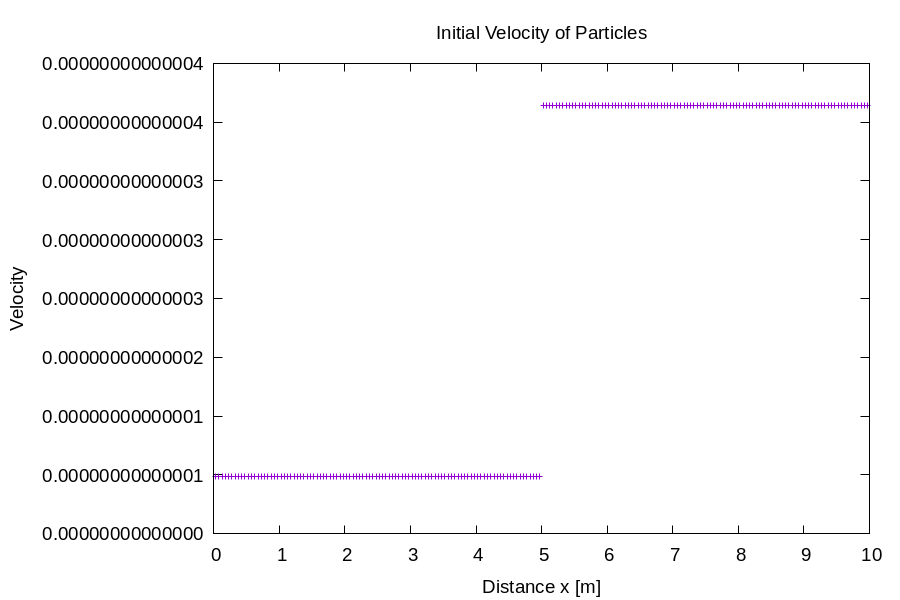
\includegraphics[width=7cm]{init-u} }}%
    \caption{Initial conditions $\rho,  u$
 }
    \label{fig:init-rho_u}
\end{figure}

\begin{figure}[H]
    \centering
    \subfloat[Left initial conditions]{{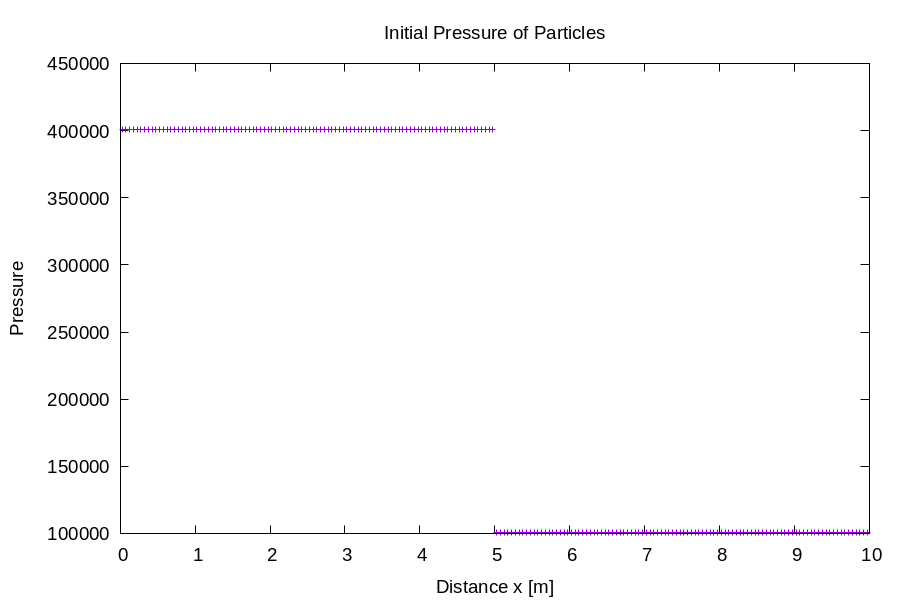
\includegraphics[width=7cm]{init-p} }}%
    \qquad
    \subfloat[Right initial conditions]{{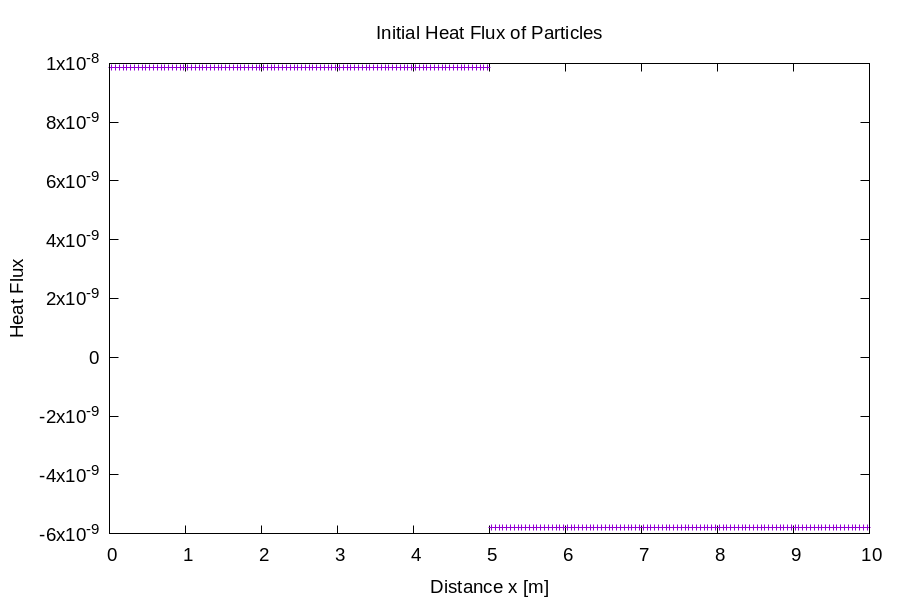
\includegraphics[width=7cm]{init-q} }}%
    \caption{Initial conditions $p, q$
 }
    \label{fig:init-p_q}
\end{figure}

\noindent
As shown in Figure \ref{fig:init-rho_u} and \ref{fig:init-p_q} the initial density calculated using the
set number density of the particles is around the $\SI{4.696}{\kilogram \per \meter^3}$
and $\SI{1.408}{\kilogram \per \meter^3}$.
The initial velocities and heat flux are near zero and the pressure is set to be near
$\SI{404.4}{\kilo \pascal}$ and $\SI{101.1}{\kilo \pascal}$.

\subsection{Results}
\begin{figure}[H]
        \centering
        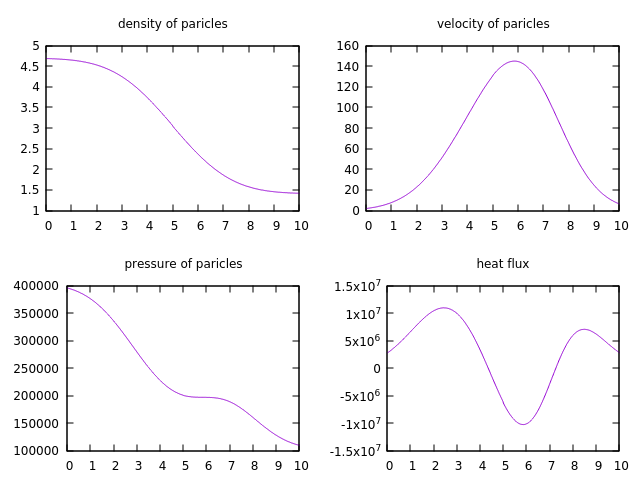
\includegraphics[width=0.8\textwidth]{tau10}
        \caption{$\tau$ = 10}
        \label{fig:tau10}
\end{figure}
\begin{figure}[H]
        \centering
        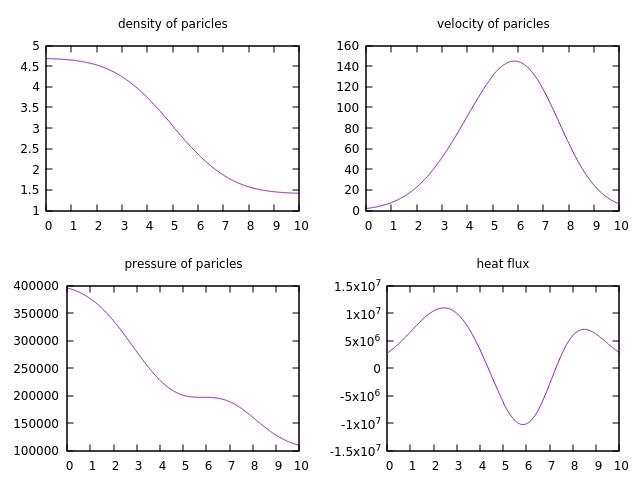
\includegraphics[width=0.8\textwidth]{tau1}
        \caption{$\tau$ = 1}
        \label{fig:tau1}
\end{figure}
\begin{figure}[H]
        \centering
        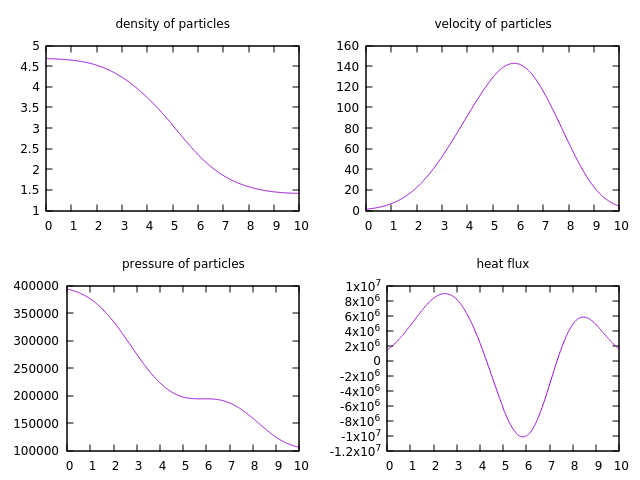
\includegraphics[width=0.8\textwidth]{tau0-01}
        \caption{$\tau$ = 0.01}
        \label{fig:tau0-01}
\end{figure}
\begin{figure}[H]
        \centering
        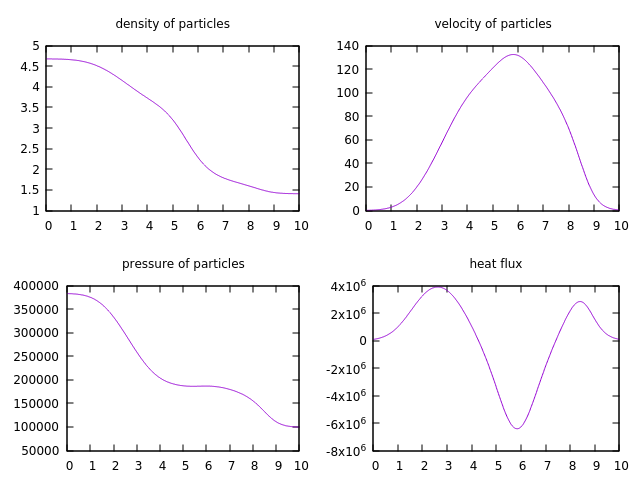
\includegraphics[width=0.8\textwidth]{tau_1e-3}
        \caption{$\tau = \SI{1e-3}{} $}
        \label{fig:tau_1e-3}
\end{figure}
\begin{figure}[H]
        \centering
        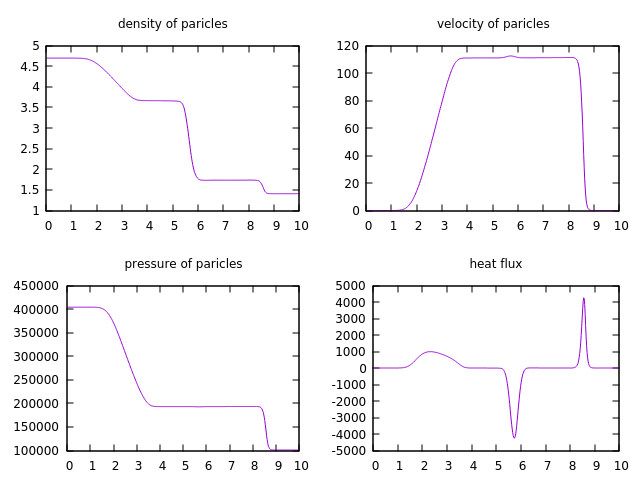
\includegraphics[width=0.8\textwidth]{tau_1e-7}
        \caption{$\tau = \SI{1e-7}{}$ }
        \label{fig:tau_1e-7}
\end{figure}

\noindent
By looking at Figures \ref{fig:tau10} - \ref{fig:tau_1e-7} we can attempt to estimate the
continuum, transition and free-molecular regimes.
In free-molecular regimes particles have little interactions with each other, we seem to be in a
free-molecular flow in between $\tau = 10$ to $\tau \approx 0.01$.
After which the flow enters a transition zone until it arrives at the continuum region near
$\tau \approx \SI{1e-7}{}$.

\noindent
In addition to the change of the fluid properties along the $x$ axis we can also
evaluate the velocity distribution at certain points along the shock tube.
Looking at the probability distribution of the particles at given points lets us
observer the most likely velocities particles are to be found at those given points.

\noindent
It is important to note that to properly capture the flow in the continuum regime the bounds of velocity
space had to be modified to $\pm \SI{5000}{\meter \per \second}$
for $\tau = \SI{1e-7}{}$.

\begin{figure}[H]
        \centering
        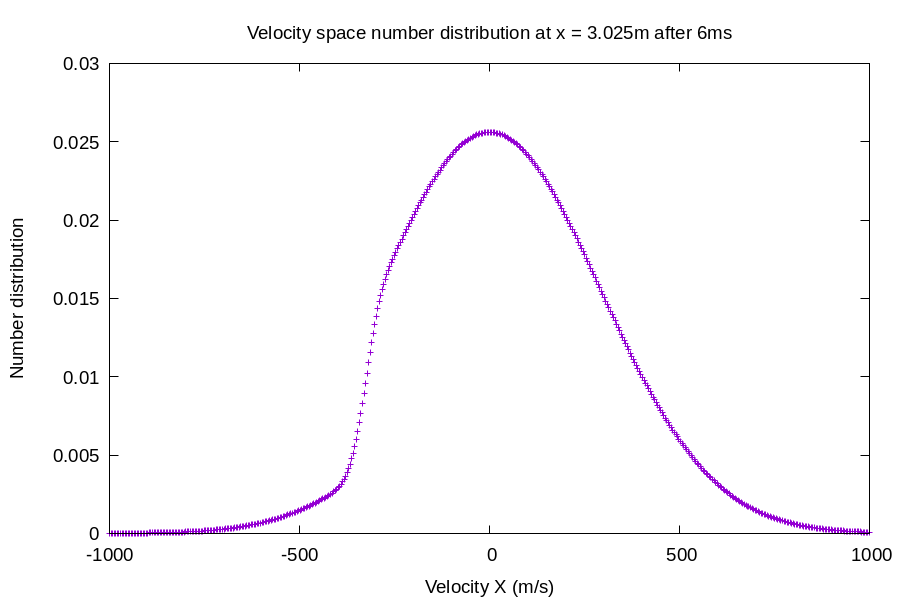
\includegraphics[width=0.8\textwidth]{left_f-t}
        \caption{Left velocity distribution at $x = \SI{3.025}{\meter}, \tau = 1.0$ }
        \label{fig:left_f-t}
\end{figure}
\begin{figure}[H]
        \centering
        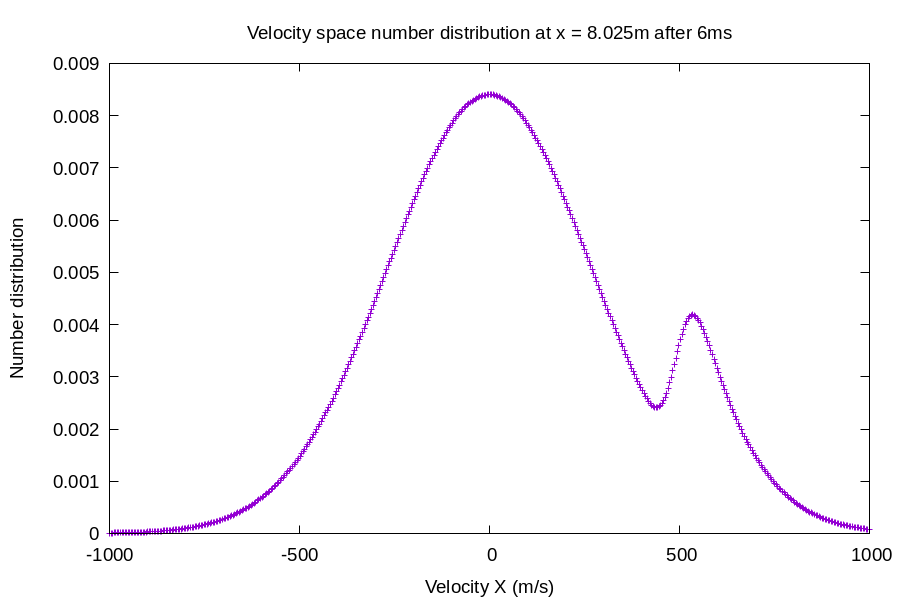
\includegraphics[width=0.8\textwidth]{right_f-t}
        \caption{Right velocity distribution at $x = \SI{8.025}{\meter}, \tau = 1.0$ }
        \label{fig:right_f-t}
\end{figure}
\begin{figure}[H]
        \centering
        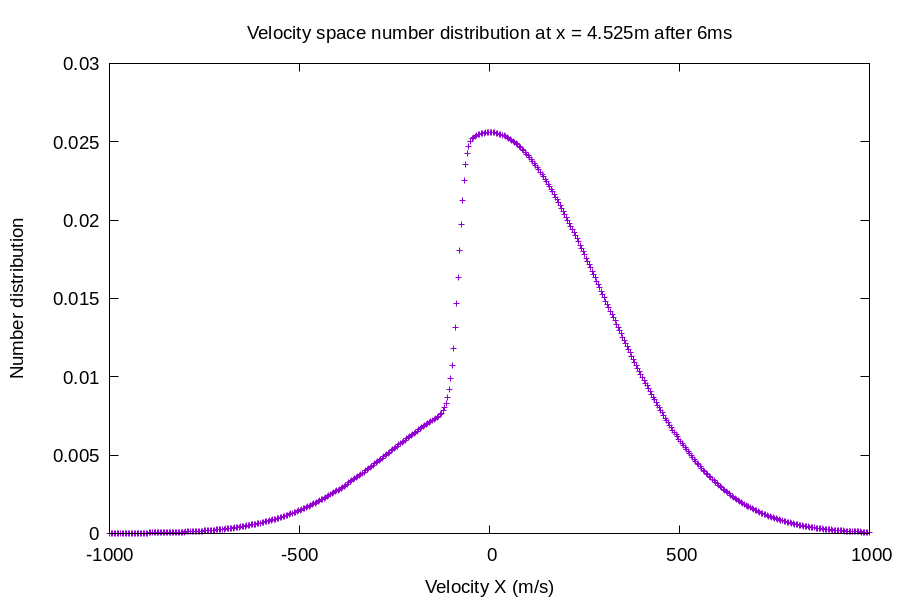
\includegraphics[width=0.8\textwidth]{center_shock-t}
        \caption{Velocity distribution near center of shock-tube, $\tau = 1.0$}
        \label{fig:center_shock-t}
\end{figure}
\begin{figure}[H]
        \centering
        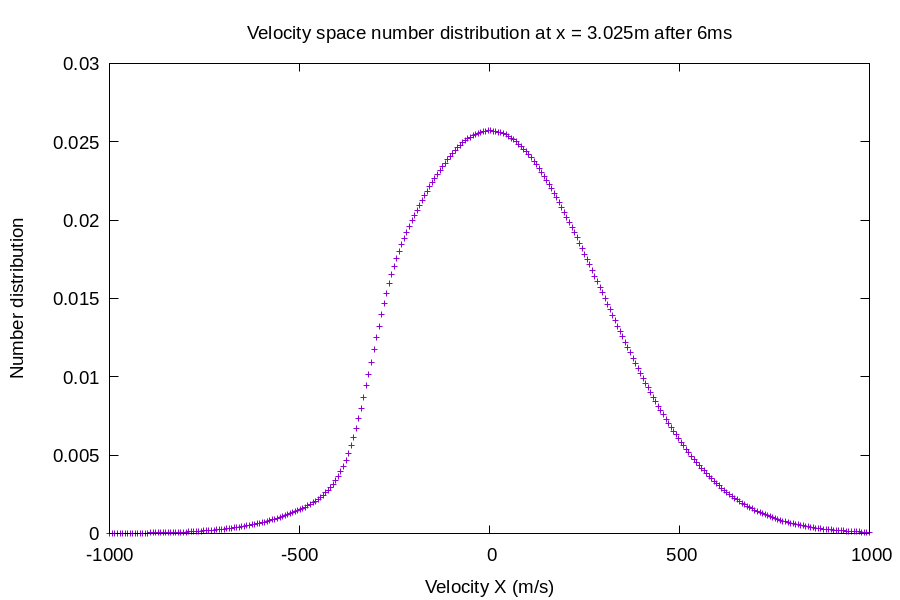
\includegraphics[width=0.8\textwidth]{left_f}
        \caption{Left velocity distribution at $x = \SI{3.025}{\meter}, \tau = \SI{1e-3}{}$ }
        \label{fig:left_f}
\end{figure}
\begin{figure}[H]
        \centering
        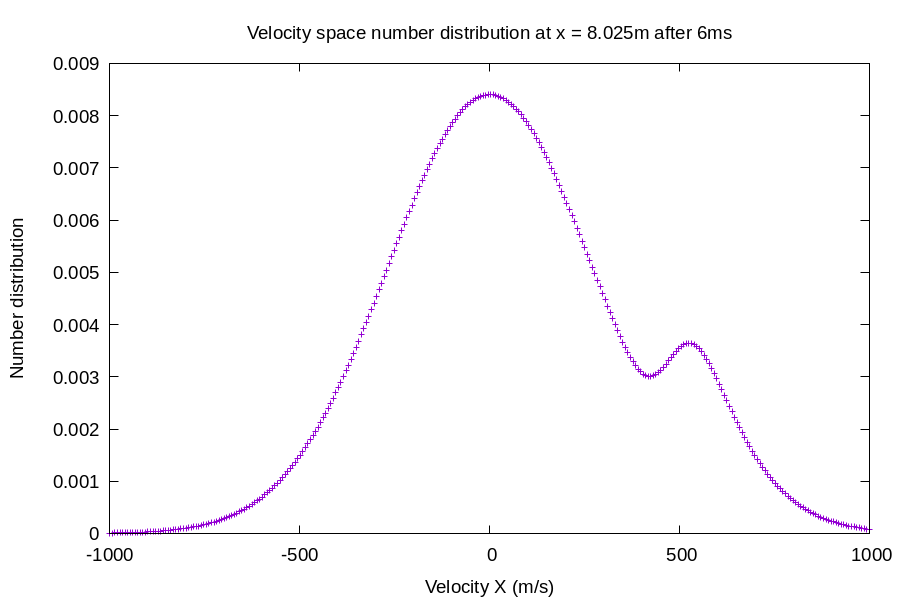
\includegraphics[width=0.8\textwidth]{right_f}
        \caption{Right velocity distribution at $x = \SI{8.025}{\meter}, \tau = \SI{1e-3}{}$ }
        \label{fig:right_f}
\end{figure}
\begin{figure}[H]
        \centering
        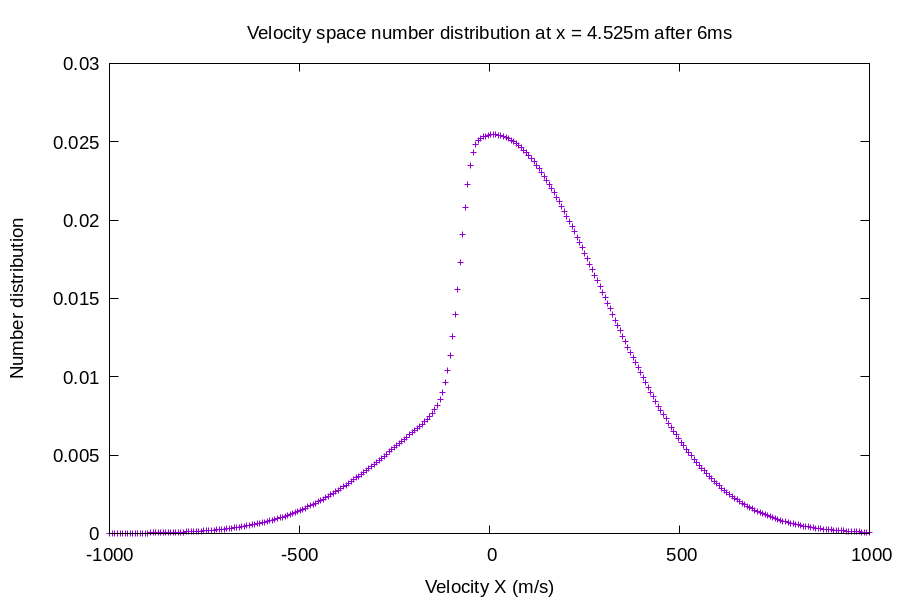
\includegraphics[width=0.8\textwidth]{center_shock}
        \caption{Velocity distribution near center of shock-tube, $\tau = \SI{1e-3}{}$}
        \label{fig:center_shock}
\end{figure}


\section{Shock-wave problem}
For this problem the up-steam conditions are set to the following
\begin{align*}
        \rho_l &= \SI{1.225}{\kilogram \per \meter^3}\\
        p_l &= \SI{101.325}{\kilo \pascal}
\end{align*}
Because we know that $\gamma = 3.0$ we can determine the speed of sound for the fluid by the following
equation.
\[
        c= \sqrt{\gamma \frac{p}{\rho}}
\]
The velocity of the fluid can then be calculated for a given Mach $M$, by the following equation.
\[
v = M \sqrt{\gamma \frac{p}{\rho}}
\]
Given that this is a normal shock we can also calculated to downstream conditions using the following
equations.
\[
        \frac{p_r}{p_l} = \frac{2 \gamma M^2 - (\gamma-1)}{\gamma+1}
\]
\[
        \frac{\rho_r}{\rho_l} = \frac{(\gamma+1)M^2}{(\gamma-1)M^2 +2}
\]
\[
        M_r^2= \frac{(\gamma -1)M^2 +2}{2\gamma M^2-(\gamma-1)}
\]
\subsection{Results}
As this is a normal shock the domain (in the $x$ direction) does not have to be really large as we are only
evaluating the conditions before and after the shock.
Because of this a domain ranging from $\SI{0}{\meter}$ to $\SI{0.5}{\meter}$ was selected.


For a mach number of $2$ the following upstream and downstream conditions were used to initially set the
domain.
\begin{center}
\begin{verbatim}
Begin shock time maching
UPSTEAM CONDITIONS
MACH:       2
Rho:        1.225kg/m^3
Pressure:   101325Pa
Velocity:   996.279m/s

DONWSTREAM CONDITIONS
Rho:        1.96kg/m^3
Pressure:   557288Pa
Velocity:   622.674m/s
\end{verbatim}
\end{center}
With $\tau = \SI{1e-7}{}$ and a final time of $tf = \SI{1e-4}{\second}$ the flow properties along the shock are the following.
\begin{figure}[H]
        \centering
        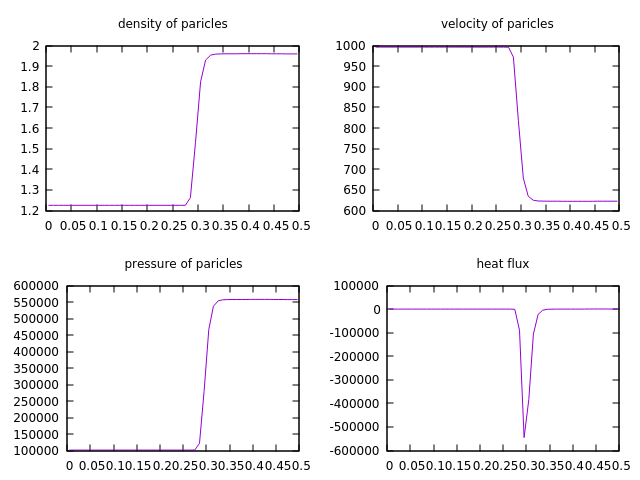
\includegraphics[width=0.8\textwidth]{mach-2-f}
        \caption{Properties along the shock, $\tau = \SI{1e-7}{}$ }
        \label{fig:mach-2-f}
\end{figure}
In addition to observing the flow properties along the shock we can also investigate the distribution
at certain points along the shock.
\begin{figure}[H]
        \centering
        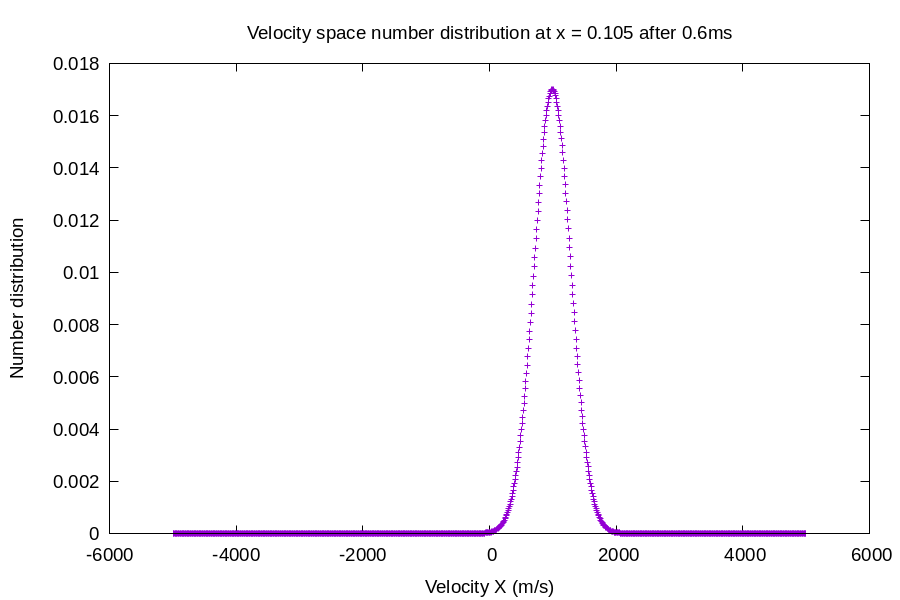
\includegraphics[width=0.8\textwidth]{left_f-m}
        \caption{Distribution at $x=0.105$ }
        \label{fig:left_f-m}
\end{figure}
\begin{figure}[H]
        \centering
        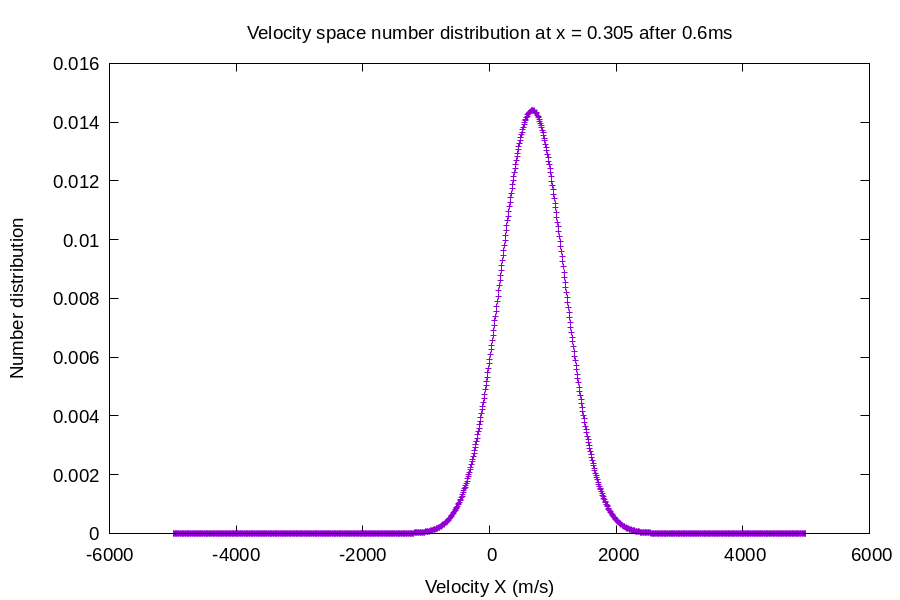
\includegraphics[width=0.8\textwidth]{center_shock-m}
        \caption{Distribution near shock at $x = 0.305$ }
        \label{fig:center_shock-m}
\end{figure}

For a mach number of $4$ the following upstream and downstream conditions were used to initially set the
domain.
\begin{verbatim}
Begin shock time maching
UPSTEAM CONDITIONS
MACH:       4
Rho:        1.225kg/m^3
Pressure:   101325Pa
Velocity:   1992.56m/s

DONWSTREAM CONDITIONS
Rho:        2.30588kg/m^3
Pressure:   2.38114e+06Pa
Velocity:   1058.55m/s
\end{verbatim}
With $\tau = \SI{1e-7}{}$ and a final time of $tf = \SI{1e-4}{\second}$ the flow properties along the shock are the following.
\begin{figure}[H]
        \centering
        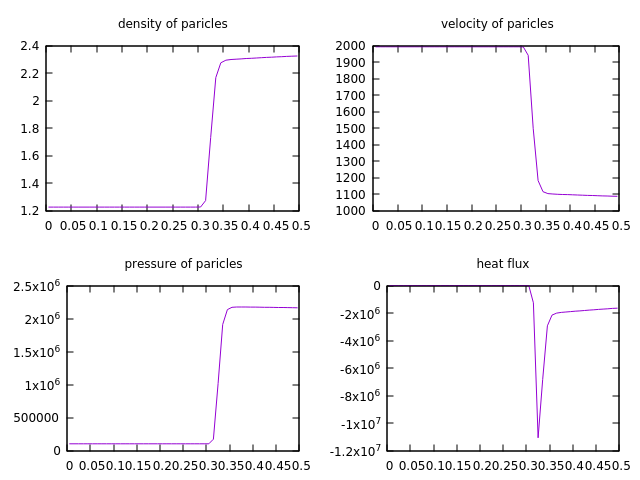
\includegraphics[width=0.8\textwidth]{mach-4-f}
        \caption{Properties along the shock, $\tau = \SI{1e-7}{}$ }
        \label{fig:mach-4-f}
\end{figure}
In addition to observing the flow properties along the shock we can also investigate the distribution
at certain points along the shock.
\begin{figure}[H]
        \centering
        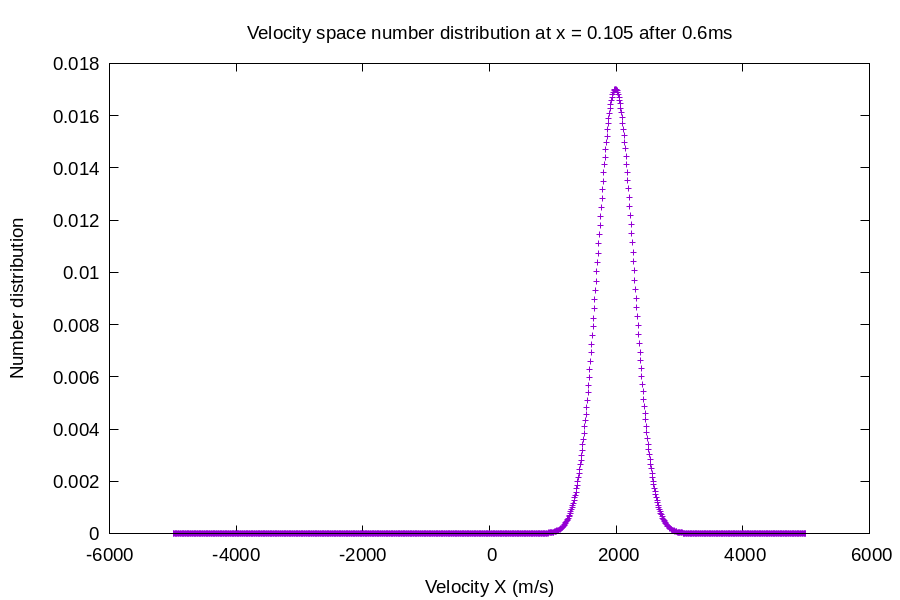
\includegraphics[width=0.8\textwidth]{left_f-m_4}
        \caption{Distribution at $x=0.105$ }
        \label{fig:left_f-m_4}
\end{figure}
\begin{figure}[H]
        \centering
        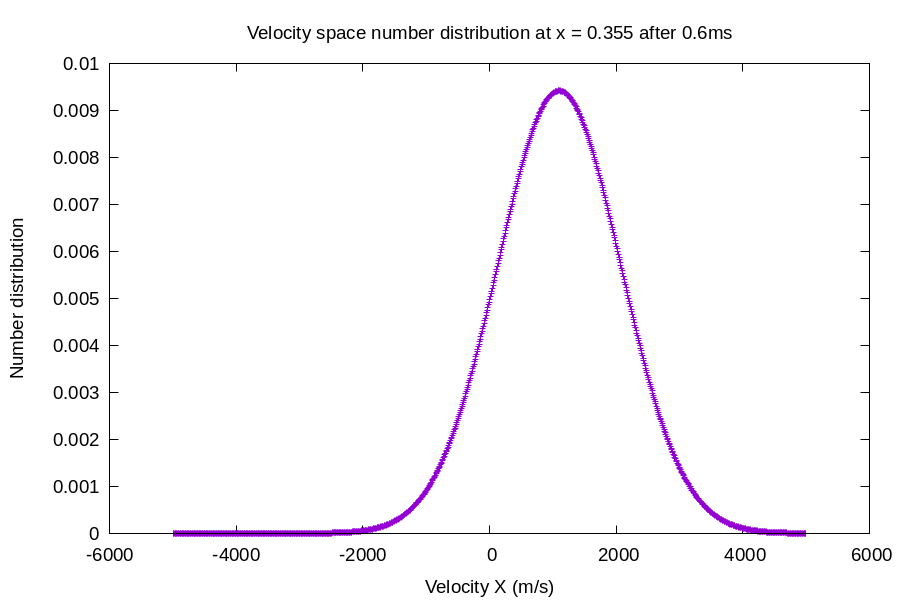
\includegraphics[width=0.8\textwidth]{center_shock-m_4}
        \caption{Distribution near shock at $x = 0.305$ }
        \label{fig:center_shock-m_4}
\end{figure}
It is important to note that as we have significantly decreased $\tau$ compared to the
problem 1 and the $\Delta x$ step in physical space we also needed to reduce
the time step $\Delta t$ to still achieve stable time marching.
Here we notice that for both distribution functions, mach $2$ and $4$ the bulk
velocity of the fluid pre-shock is held together very closely around its initial velocity.
Where as at the shock and after the shock the velocity distribution is much more spread out.
Additionally pre-shock values have an almost zero probability of a velocity in the
negative $x$ direction.
After the shock the is a small amount of particles that have a negative velocity.




\end{document}
